\documentclass[draft, 12pt]{article}
\usepackage[english]{babel}
\usepackage[final]{graphicx}
\usepackage{multirow}
\usepackage{color}
\graphicspath{ {figures/} }
\DeclareGraphicsExtensions{.png}

\newcommand{\cc}[1]{\textcolor{red}{#1}}

\title{Seismic parameter estimation and the Canadian crust}
\author{Ben Postlethwaite}

%% ------------------------------------------------------------------------ %%
\begin{document}

\begin{abstract}

\end{abstract}

%% -----------------------------------------------%%
\section{Introduction}

  Seismic studies of the Canadian continental crust predominately analyze specific geological features or regions rather than taking a comprehensive and comparative inter-regional analysis. The primary reason for this is the poor resolution afforded by the seismic networks currently and historically deployed across Canada. The Canadian continental landmass is composed of at least fifteen large geological provinces as recognized by the Geological Survey of Canada (GSC). Each of these regions is itself complex and heterogeneous and often larger than most European nations. On top of this there is poor seismic coverage, roughly one seismic station per 25,000 $km^2$. Many of these stations are clustered near areas of geologic interest such as the Cascadia Subduction zone or population and research centres such as Southern Ontario or areas of significant resource interest like the diamondiferous Great Slave Lake area. This leaves vast areas of the Canadian landmass completely unsampled. Despite these limitations, a low resolution comprehensive and comparative study is still feasible for some of the geological regions comprising the Canadian continental crust. Direct comparison between the bulk average seismic properties of geological regions and between aggregated regions and global averages provide some new insight into the crustal composition of the Canadian landmass. The accumulated dataset also affords investigations into variations of bulk crustal parameters such as Poisson's Ratio and crustal thickness with age and tectonic environment as well as some basic statistical data on interesting crustal features.

  This paper presents a comparative tour through the dataset accumulated from processing more than a decade worth of data from all available Canadian seismic stations. It begins with a discussion of the raw data itself followed by a review of the receiver function method and a more detailed explanation of the inversion algorithms used to produce the dataset. Three previous publications utilizing similar processing schemes provide unique subsets of data to compare with the values computed in this survey for quality assurance. ...


\subsection{Geological and tectonic summary}


\subsection{Previous geophysical studies}

%% -----------------------------------------------%%
\section{Data and methods}
  Analysis of bulk Canadian continental crust requires estimates of crustal properties such as seismic-wave velocity and crustal thickness. This study draws on three sources for these crustal properties. The first and primary source for these estimates are data computed by processing raw seismograms into receiver functions and then inverting these RF's for parameter estimates. The other two datasets, the statistically compiled Crust 2.0 dataset and a compilation of pre-processed active source data, are used to qualify and compare with the primary dataset.

\subsection{Teleseismic Data Set}

  The primary data utilized in this study are computed from teleseismic P-wave seismograms representing discrete seismic events. These events are comprised of seismic records representing more than 700 earthquake sources occurring between the years 2000 and 2012 at 343 broadband seismic stations across Canada. Seismic stations are selected from all available regional and national networks including CNSN, Polaris, FedNor and Chasme. Events are filtered by the epicentral distance from source to receiver with only the events within a 30 to 100 degree window being included. Seismic events are further filtered by hand picking those with reasonable signal to noise ratio and of sufficient impulsiveness that arrival times can be accurately measured. After selection and filtering more than 80,000 events are available for further processing.

  The first stage of processing requires the transformation of teleseismic data into receiver functions. In its generic form this transformation involves deconvolving an approximation of the earthquake source from channels representing ground motion. The resulting waveform contains discrete pulses corresponding to the arrivals of S-wave energy scattered from subsurface discontinuities. Resolving these peaks is essential to the success of the following inversion, therefore it is advantageous to rotate the seismogram components to separate the P and S wave energy. This is accomplished by first rotating the N and E coordinates into radial and transverse dimensions and then performing a wave field decomposition on the radial and vertical channels [Bostock, 1998]. The direct arrival of the signal on the resulting P wave component is used as an approximation to the source function as P waves are simpler and have a response closer to that of a delta function. This windowed source coda is deconvolved from the S wave component computed from the wave field decomposition.

  An $L_2$ frequency domain deconvolution approach is used which has the advantages of computational efficiency as well as not requiring any assumptions about the noise in the data. This method performs a simultaneous deconvolution of $N$ seismograms sharing a similar slowness to compute a single impulse response or receiver function $r(t)$.
% Deconvolution equations
\begin{equation}
  r(t) = F^{-1} \left[ G(\omega) \right] = F{^-1}
 \left[ \frac {\sum_n^N S_n(\omega)P_n^*(\omega)} {\sum_n^N P_n(\omega)P_n^*(\omega) + \delta} \right ],
\end{equation}

where $F^{-1}$ is the inverse Fourier transform, $S_n$ represents the $n^{th}$ S wave component, $P_n$ is the windowed P wave component, $^*$ denotes the complex conjugate and $\delta$ is the regularization parameter controlling the trade off between model smoothness and data misfit. The parameter $\delta$ is chosen programatically by minimizing the general cross validation function $GCV(\delta)$ which is given by

\begin{equation}
  GCV(\delta) = \frac {\sum_n^N\sum_m^M \left( S_n(\omega_m) - P_n(\omega_m)G(\omega_m) \right)^2 }
                      { \left( NM - \sum_m^M X(\omega_m) \right)^2 },
\end{equation}

where

\begin{equation}
  X(\omega) = \frac {\sum_n^N P_n(\omega)P_n^*(\omega)} {\sum_n^N P_n(\omega)P_n^*(\omega) + \delta},
\end{equation}

and $\omega_m$ is the $m^{th}$ frequency bin in the discrete Fourier transform.

  All resulting receiver functions, $r(t)$, are filtered between 0.04Hz and 3.0Hz.



\subsection{Vp/Vs method} \label{section:VpVsMethod}

\begin{figure}
  \centering
    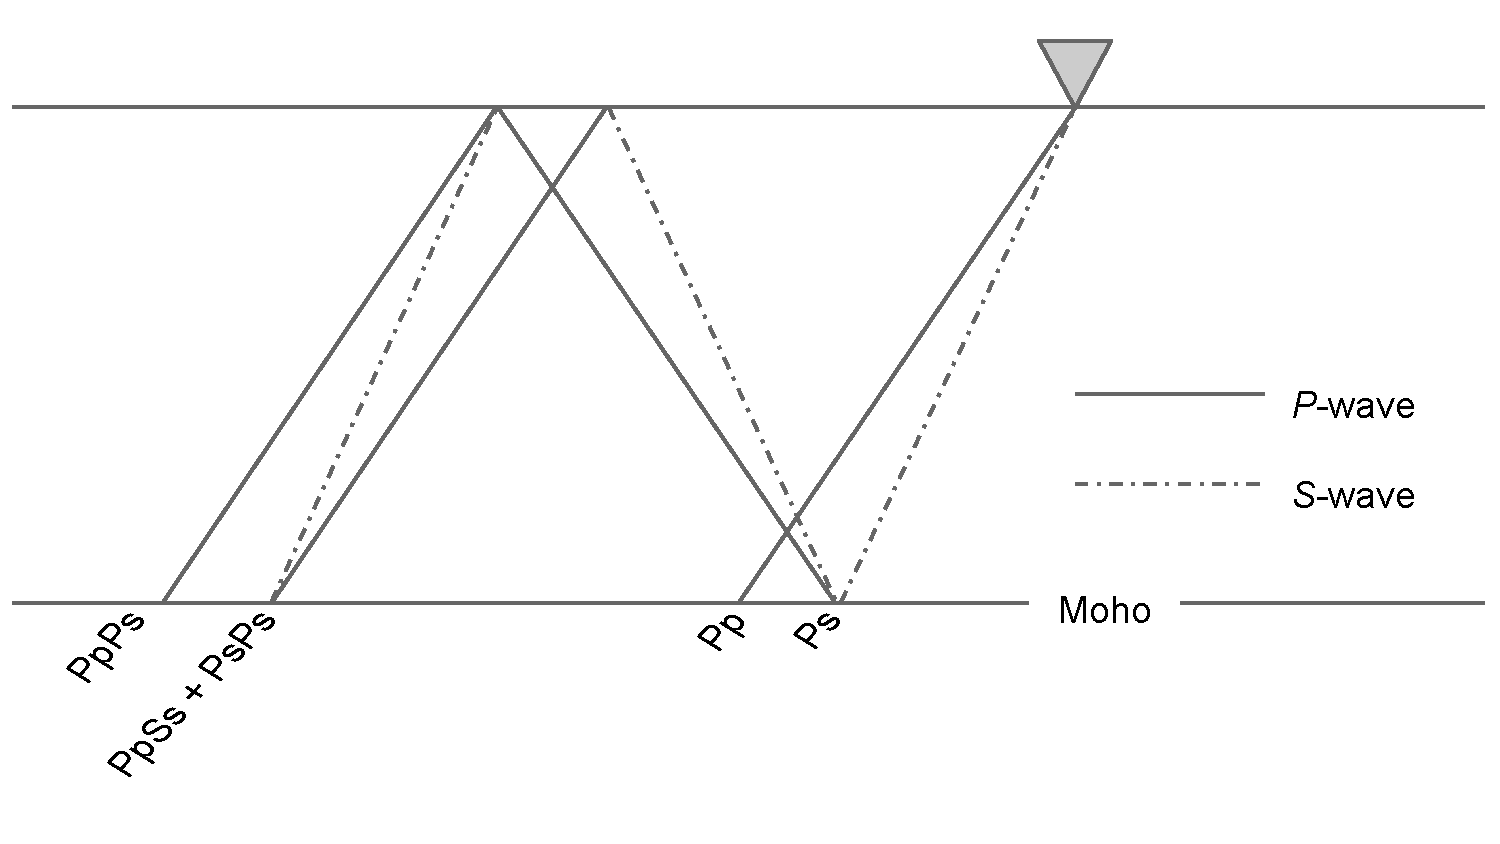
\includegraphics[width=\textwidth]{reflectedPhases}
  \caption{Schematic diagram illustrating geometry of phases for the velocity contrast representing the Moho}
  \label{fig:reflectedPhases}
\end{figure}


  A well tested and widely published method for extracting the ratio, $R=\frac{V_P}{V_S}$, where $V_P$ is P-wave velocity and $V_S$ is S-wave velocity and crustal thickness, or depth to Moho, $H$, is outlined by Zhu and Kanamori [2000], hereafter ZK. This method takes advantage of the differential arrival times between the S-wave reflected phases $Ps$, $PpPs$ $PsPs$, $PpSs$ and $PsSs$ and the direct P-wave arrival $Pp$ (Fig \ref{fig:reflectedPhases}). Note that $PsPs$ and $PpSs$ have an equal number of $P$ and $S$ phases, and the energy for these two phases arrive simultaneously and are indistinguishable. For a range of slowness values, $p$, the differential arrival times, $t(p)$, trace moveout curves for each phase arrival given by

% Travel time equations
\begin{equation} \label{eq:tps}
t_{Ps}(p_i)=H \left[ \sqrt{ \left(\frac{R}{V_P}\right)^2 - p_i^2} - \sqrt{\frac{1}{V_P^2} - p_i^2} \right]
\end{equation}

\begin{equation}
t_{Pps}(p_i)=H \left[ \sqrt{ \left(\frac{R}{V_P}\right)^2 - p_i^2} + \sqrt{\frac{1}{V_P^2} - p_i^2} \right]
\end{equation}

\begin{equation}
t_{Pss}(p_i)= 2H  \sqrt{ \left(\frac{R}{V_P}\right)^2 - p_i^2}
\end{equation}

where $p_i$ is the slowness for the $i^{th}$ receiver function. Since strong reflected phases occur at sharp velocity contrasts, the Moho, the boundary targeted by ZK, tends to be well represented on most RF's.

  The travel time equations demand an apriori assumption on crustal P-wave velocity, $V_P$, and will trade-off to some degree with crustal thickness $H$. For this study, each station is assigned a $V_P$ value corrisponding to the Crust 2.0 value for the $2^o$ containing cell. In the specific cases where data is being compared to previously published results for quality control, $V_P$  values are chosen to match the values in the published study.

\begin{figure}
  \centering
    \includegraphics[width=\textwidth]{kinematicRvsH}
  \caption{Kinematic curves traced out by the stacking function, $s(H,R)$, corrisponding to the mapping of fixed travel times $t_{Ps}$, $t_{PpPs}$ and $t_{PsPs}$ into $H$ and $R$ space.}
  \label{fig:kinematicRvsH}
\end{figure}


  For a range of candidate models of $R$ and $H$ the RF's are stacked along trial moveout curves. During the stacking procedure each phase is assigned a weight to account for a general trend in the quality of the phases, with direct arrival usually carrying the best signal followed by $PpPs$ and $PpSs$. The weights chosen during the stacking are $w1 = 0.5$, $w2 = 0.3$ , $w3 = -0.2$ for the $Ps$, $PpPs$ and $PpSs$ phases respectively. A negative weight for the combined $PpSs$ and $PsPs$ phases is required as the polarity of the signal is reversed. Semblance weighting [Eaton, 2006] is employed to reduce the effect of spurious large amplitude noise in the data. The semblance function assigns a weight between zero (incoherent noise) and one (coherent signal). The stacking function is therefore defined as

\begin{equation}  \label{eq:stack}
s(H,R) = \sum_{j=1}^{3} S_j \sum_{i=1}^N w_jr_i(t_j)
\end{equation}

where

\begin{equation}
S_j(H,R) = \frac {\left[ \sum_{i=1}^N r_i(t_j) \right]^2}
                 { \sum_{i=1}^N r_i^2(t_j) }
\end{equation}

and $S_j$ is the semblance weight for the $j^{th}$ phase, time $t_j$ is calculated from the corrisponding travel time function for a given $H$, $R$ as a function of slowness $p_i$ and $N$ is the number of receiver functions. Multiplying by the semblance weighting sharpens the stacked image, $s(H,R)$, and exhibits better resolution when selecting between stacked models. The function $s(H,R)$ can be thought of as a transformation that maps the $Ps$, $PpPs$ and $PpSs+PsPs$ pulses of the receiver function, $r(t)$,  into $R$ and $H$ space as positive bands, via Eq. \ref{eq:stack}. Constructive interference where these bands intersect will produce a maximum in the stacking function (Fig \ref{fig:kinematicRvsH}). The model, $R$ and $H$, which produce this maximum provides the best estimate for the bulk crustal parameters for a given seismic station. The elongate shape about the point of intersection, with the long axis tilted mostly in the $R$ coordinate, conveys the inherent trade-off between $R$ and $H$ and the lower resolution exhibited by the seismic velocity ratio $R$.

\subsection{Full Gridsearch Method}

  Owing to increasing computational availability it is now reasonably efficient to extend the ZK approach and perform the stack along a range of all three seismic parameters, $V_P$, $R$ (therefore by definition $V_S$) and $H$. This has the advantage of not requiring an assumption on $V_P$ and should produce more accurate estimates, especially above crustal units with anomalous $V_P$. The inherent trade-off between $V_P$ and $R$ is limited, offering reasonable resolution between the two parameters. However, a significant trade-off between $V_P$ and $H$, which is a source of significant correlated error, requires that recovery of $V_P$ should be attempted only in cases where high frequency and high signal-to-noise ratio signals are present in the receiver function data. [[ Could go into more depth here, show the kinematic curves and poor trade-off between $V_P$ and $R$, Figure showing correlation between $V_P$ and $H$]]

  These trade-offs, along with other sources of error such as low signal-to-noise signals resulting from complex geology, are quantified by bootstrap resampling [Efron and Tibshirani, 1986]. Estimates are reprocessed using a random selection of receiver functions, with replacement, 1024 times. An estimate for the error is computed by taking the standard deviation from these trial runs.

\subsection{Additional data}
   Accompanying the processed estimates are data from controlled source experiments collected and compiled from GSC (Geological Survey of Canada) references by Walter Mooney (personal communication, 2012). This data provides $V_P$ and a few $V_S$ estimates for hundreds of experiment locations across Canada, many along traversals across geological provincial boundaries, faults and discontinuities. Some of these data are located within close enough proximity to seismic stations being utilized in this study that they may be used to compare with the $V_P$ and $V_S$ estimates resulting from the full parameter gridsearch.

  Whereas the active source data provide high resolution values at specific sites, the Crust 2.0 model, a global dataset widely cited in academic literature, provides complete coverage across Canada with an attendant trade-off in resolution. The data includes estimates of $V_P$ and $V_S$ for $2^o$ longitude and latitude cells as well as information regarding sedimentary thickness and crustal depth. While Crust 2.0 source data is a superset of the aforementioned active source data, the crustal model is also composed of statistically aggregated data from geographically distant but geologically similar regions. It therefore forms a unique dataset well suited for comparison with the crustal estimates calculated in this study.

%% -----------------------------------------------%%
\section{Results}

\subsection{Comparisons}

  Several published regional studies utilizing the methods outlined in section \ref{section:VpVsMethod} provide parameter estimates for $R$ and $H$ for regionally grouped subsets of Canadian seismic stations. Comparisons between estimates for particular seismic stations are made for those values which have a corresponding standard error in $R$ of less than 0.06. For each study under comparison, data is reprocessed to use the $V_P$ chosen by the study authors and both correlation and mean difference are calculated (Table \ref{table:comparison}).

  A comprehensive study in the Hudson Bay region of the Canadian Shield [Thomson et. al., 2010] employs data from 35 stations, of which, 27 stations share an error acceptable for comparison in both datasets. There is strong correlation, 0.97, between crustal thickness values (Fig \ref{fig:thompsonCompH}). The velocity ratio data has a lower correlation of 0.49 (Fig \ref{fig:thompsonCompR}) and a mean difference of 0.02. As indicated in section \ref{section:VpVsMethod} there is less resolution in $R$ so the lower correlation for this parameter is not unexpected.

 Another study conducted in the Grenville Orogen [Eaton et al., 2006] utilizes data from 29 stations, with two stations being excluded due to low quality and high error. Again, there is strong correlation in $H$, 0.89, and lower correlation in $R$, 0.56 (Figs \ref{fig:eatonCompH}, \ref{fig:eatonCompR}). The mean difference in $R$ between the two datasets is 0.04.


\begin{table}
  \begin{tabular}{ l l l l l l }
    \cline{3-6}
    & & \multicolumn{2}{ c }{Correlation} & \multicolumn{2}{ c }{Mean Difference} \\
    \hline
    Study Authors & Num. of Stns & $H$ & $R$ & $H$(km) & $R$ \\
    \hline
    Thompson et. al. (2010)   & 0.97 & 0.49 & 3.36 & 0.024 \\
    Eaton et. al. (2006)      & 0.90 & 0.61 & 2.65 & 0.04  \\
    Darbyshire et. al. (2007) & 0.95 & 0.43 & 4.16 & 0.39  \\
    \hline
  \end{tabular}
  \caption{Comparison of $R$ and $H$ estimates with three published studies}
\label{table:comparison}

\end{table}


\begin{figure}
  \centering
    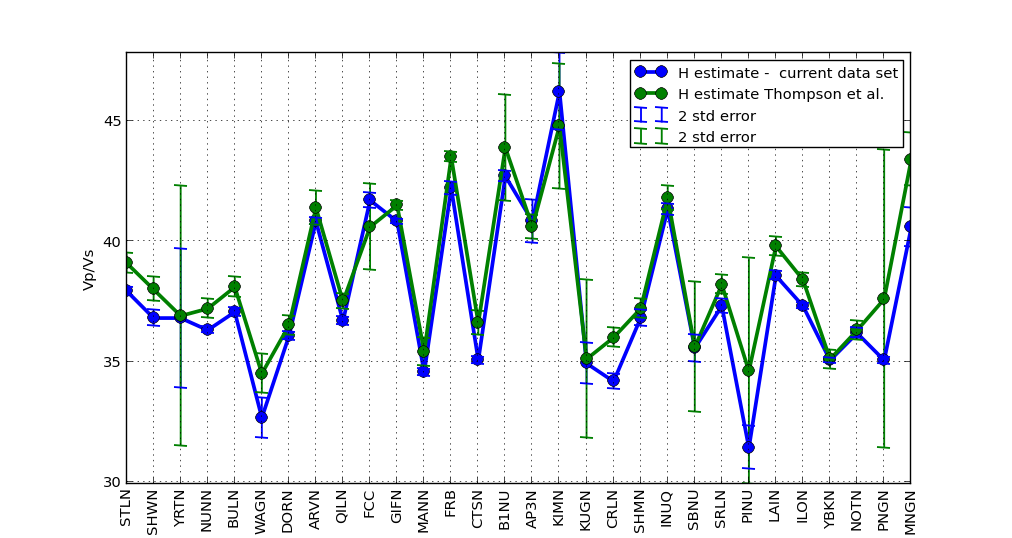
\includegraphics[width=\textwidth]{thompsonComparisonH}
  \caption{Comparison of crustal thickness $H$ data from this study with data from Thompson et. al. (2010). Data shows a Pearson correlation of 0.95}
  \label{fig:thompsonCompH}
\end{figure}

\begin{figure}
  \centering
    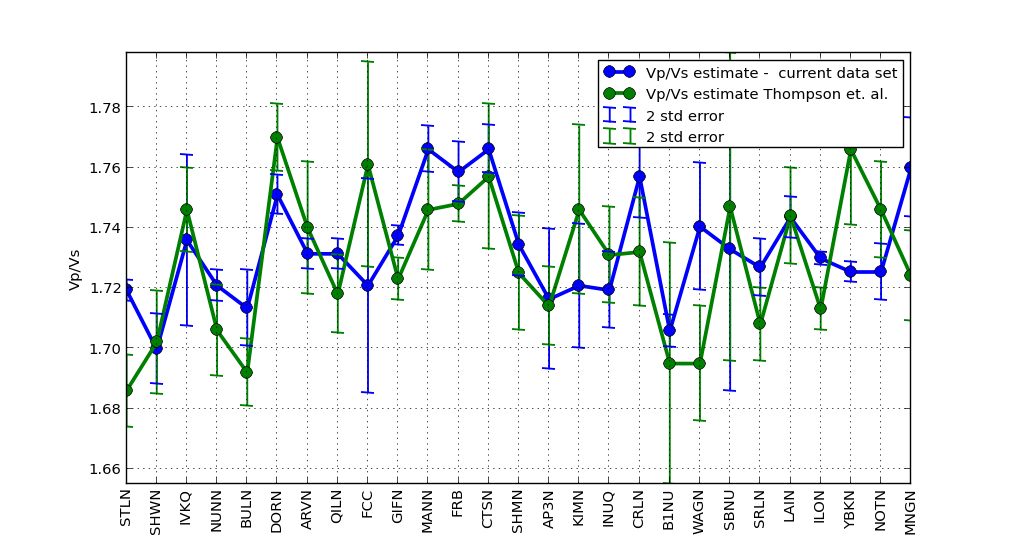
\includegraphics[width=\textwidth]{thompsonComparisonR}
  \caption{Comparison of $V_P / V_R$ data from this study with data from Thomspson et. al. (2010). Data shows a Pearson correlation of 0.5}
  \label{fig:thompsonCompR}
\end{figure}

\begin{figure}
  \centering
    \includegraphics[width=\textwidth]{eatonComparisonH}
  \caption{Comparison of crustal thickness $H$ data from this study with from Eaton et. al. (2010). Data shows a Pearson correlation of 0.95}
  \label{fig:eatonCompH}
\end{figure}

\begin{figure}
  \centering
  \includegraphics[width=\textwidth]{eatonComparisonR}
  \caption{Comparison of $V_P / V_R$ data from this study with data from Eaton et. al. (2010). Data shows a Pearson correlation of 0.5}
  \label{fig:eatonCompR}
\end{figure}

\begin{figure}
  \centering
  \includegraphics[width=\textwidth]{darbyshireComparisonH}
  \caption{Comparison of crustal thickness $H$ data from this study with data from Darbyshire et. al. (2010). Data shows a Pearson correlation of 0.95}
  \label{fig:darbyshireCompH}
\end{figure}

\begin{figure}
  \centering
  \includegraphics[width=\textwidth]{darbyshireComparisonR}
  \caption{Comparison of $V_P / V_R$ data from this study with data from Darbyshire et. al. (2010). Data shows a Pearson correlation of 0.5}
  \label{fig:darbyshireCompR}
\end{figure}



\begin{figure}
  \centering
  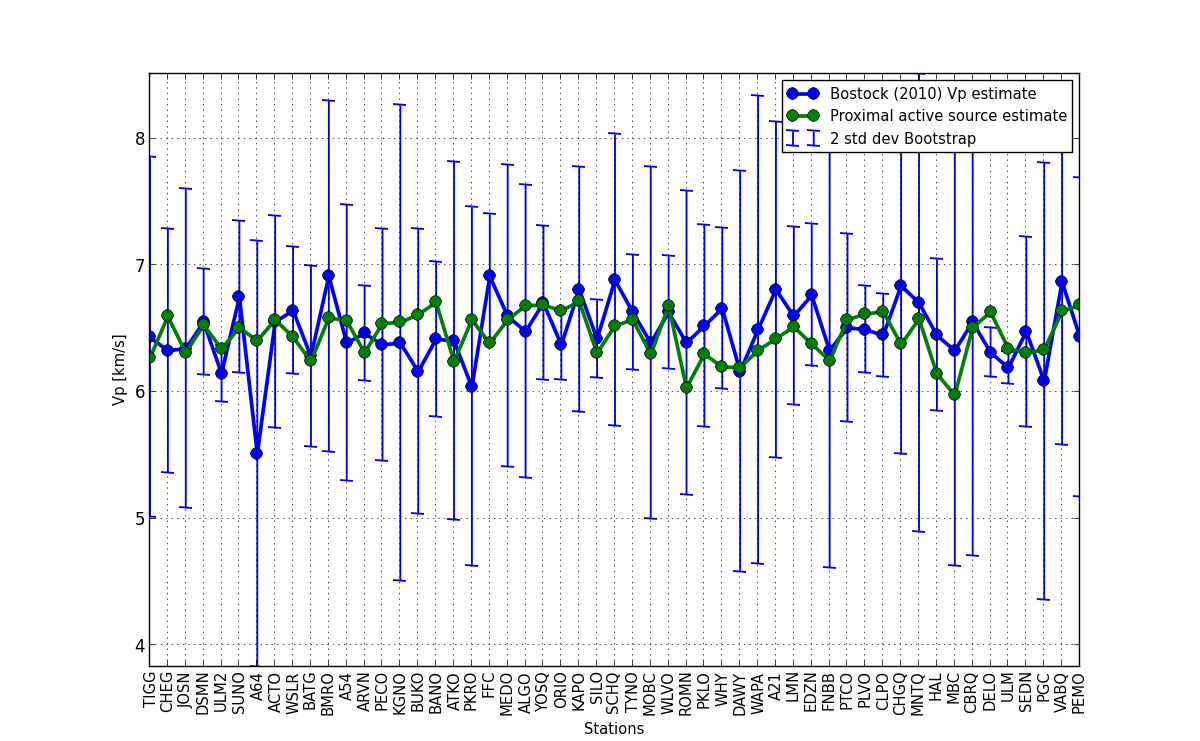
\includegraphics[width=\textwidth]{activeSourceComparison}
  \caption{Comparison of $V_P$ estimates from the MB algorithm with active source $V_P$ recordings. Stations selected if active source experiment locations within 1 degree of latitude / longtitude.}
  \label{fig:activeComp}
\end{figure}

\subsection{Regional Bulk Crustal Parameters}
(MAY NOT INCLUDE)
\begin{itemize}
  \item Jump in crustal thickness over the fault as you go from the Slave to the Rae or Churchill Province.
  \item Trend in Southern Ontario as we move north and up the St Lawrence Seaway.
  \item Appears to be secular variation in the North Eastern Churchill. As we move North and East we have thickening of continental crust.
\end{itemize}


\begin{figure}
  \centering
  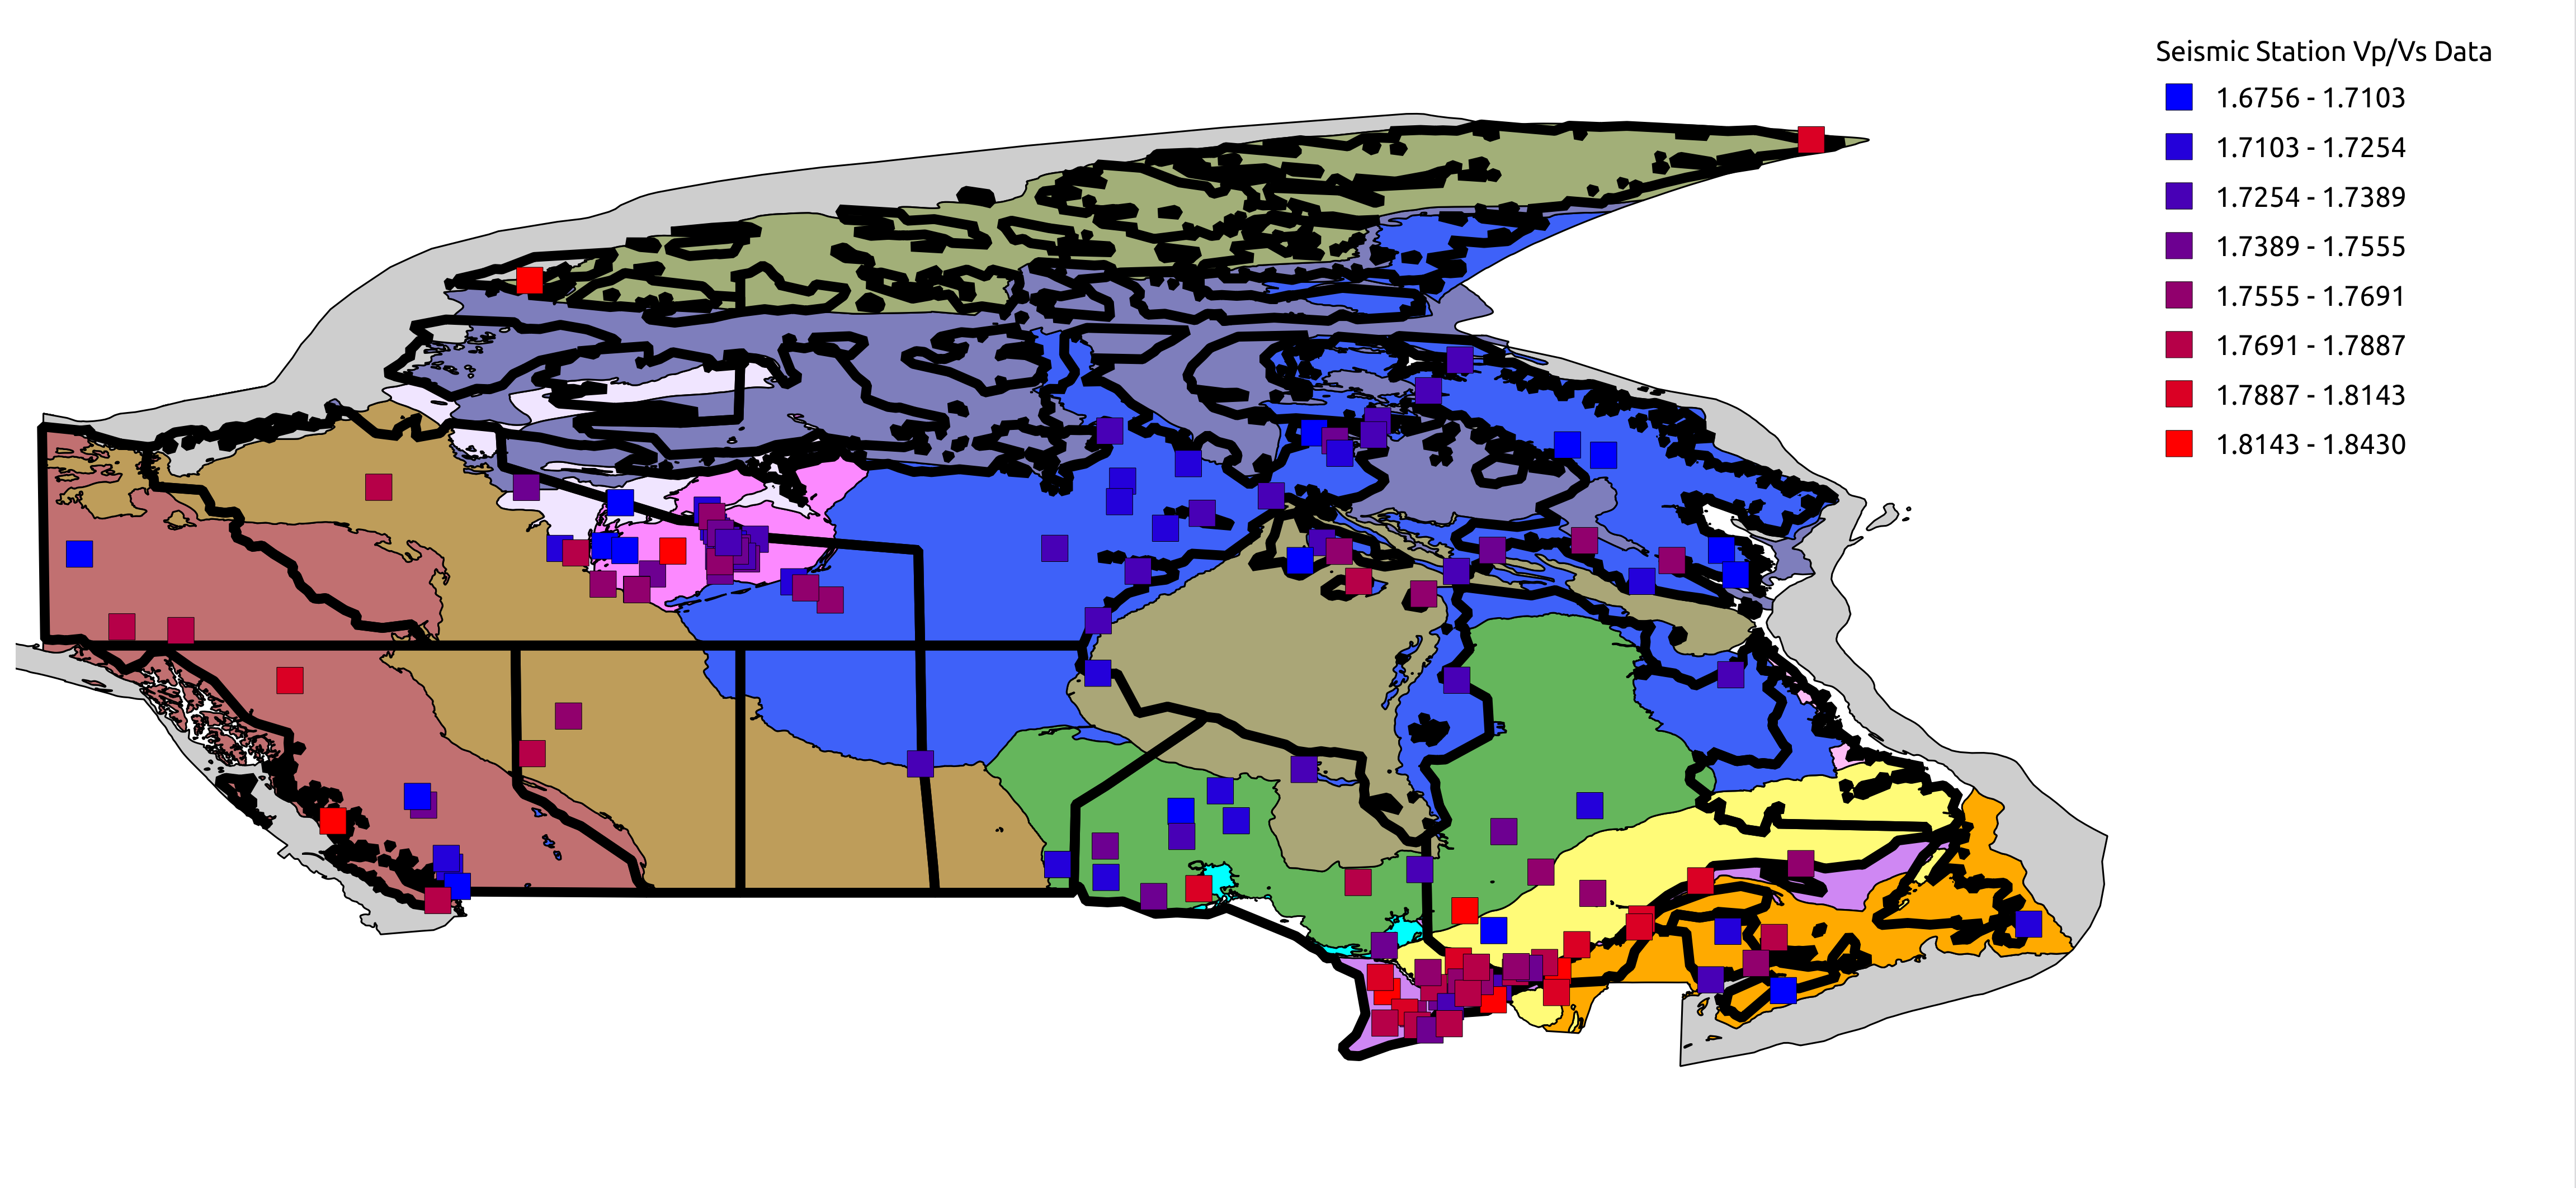
\includegraphics[width=\textwidth]{VpVsMap}
  \caption{}
  \label{fig:VpVsMap}
\end{figure}

\begin{figure}
  \centering
  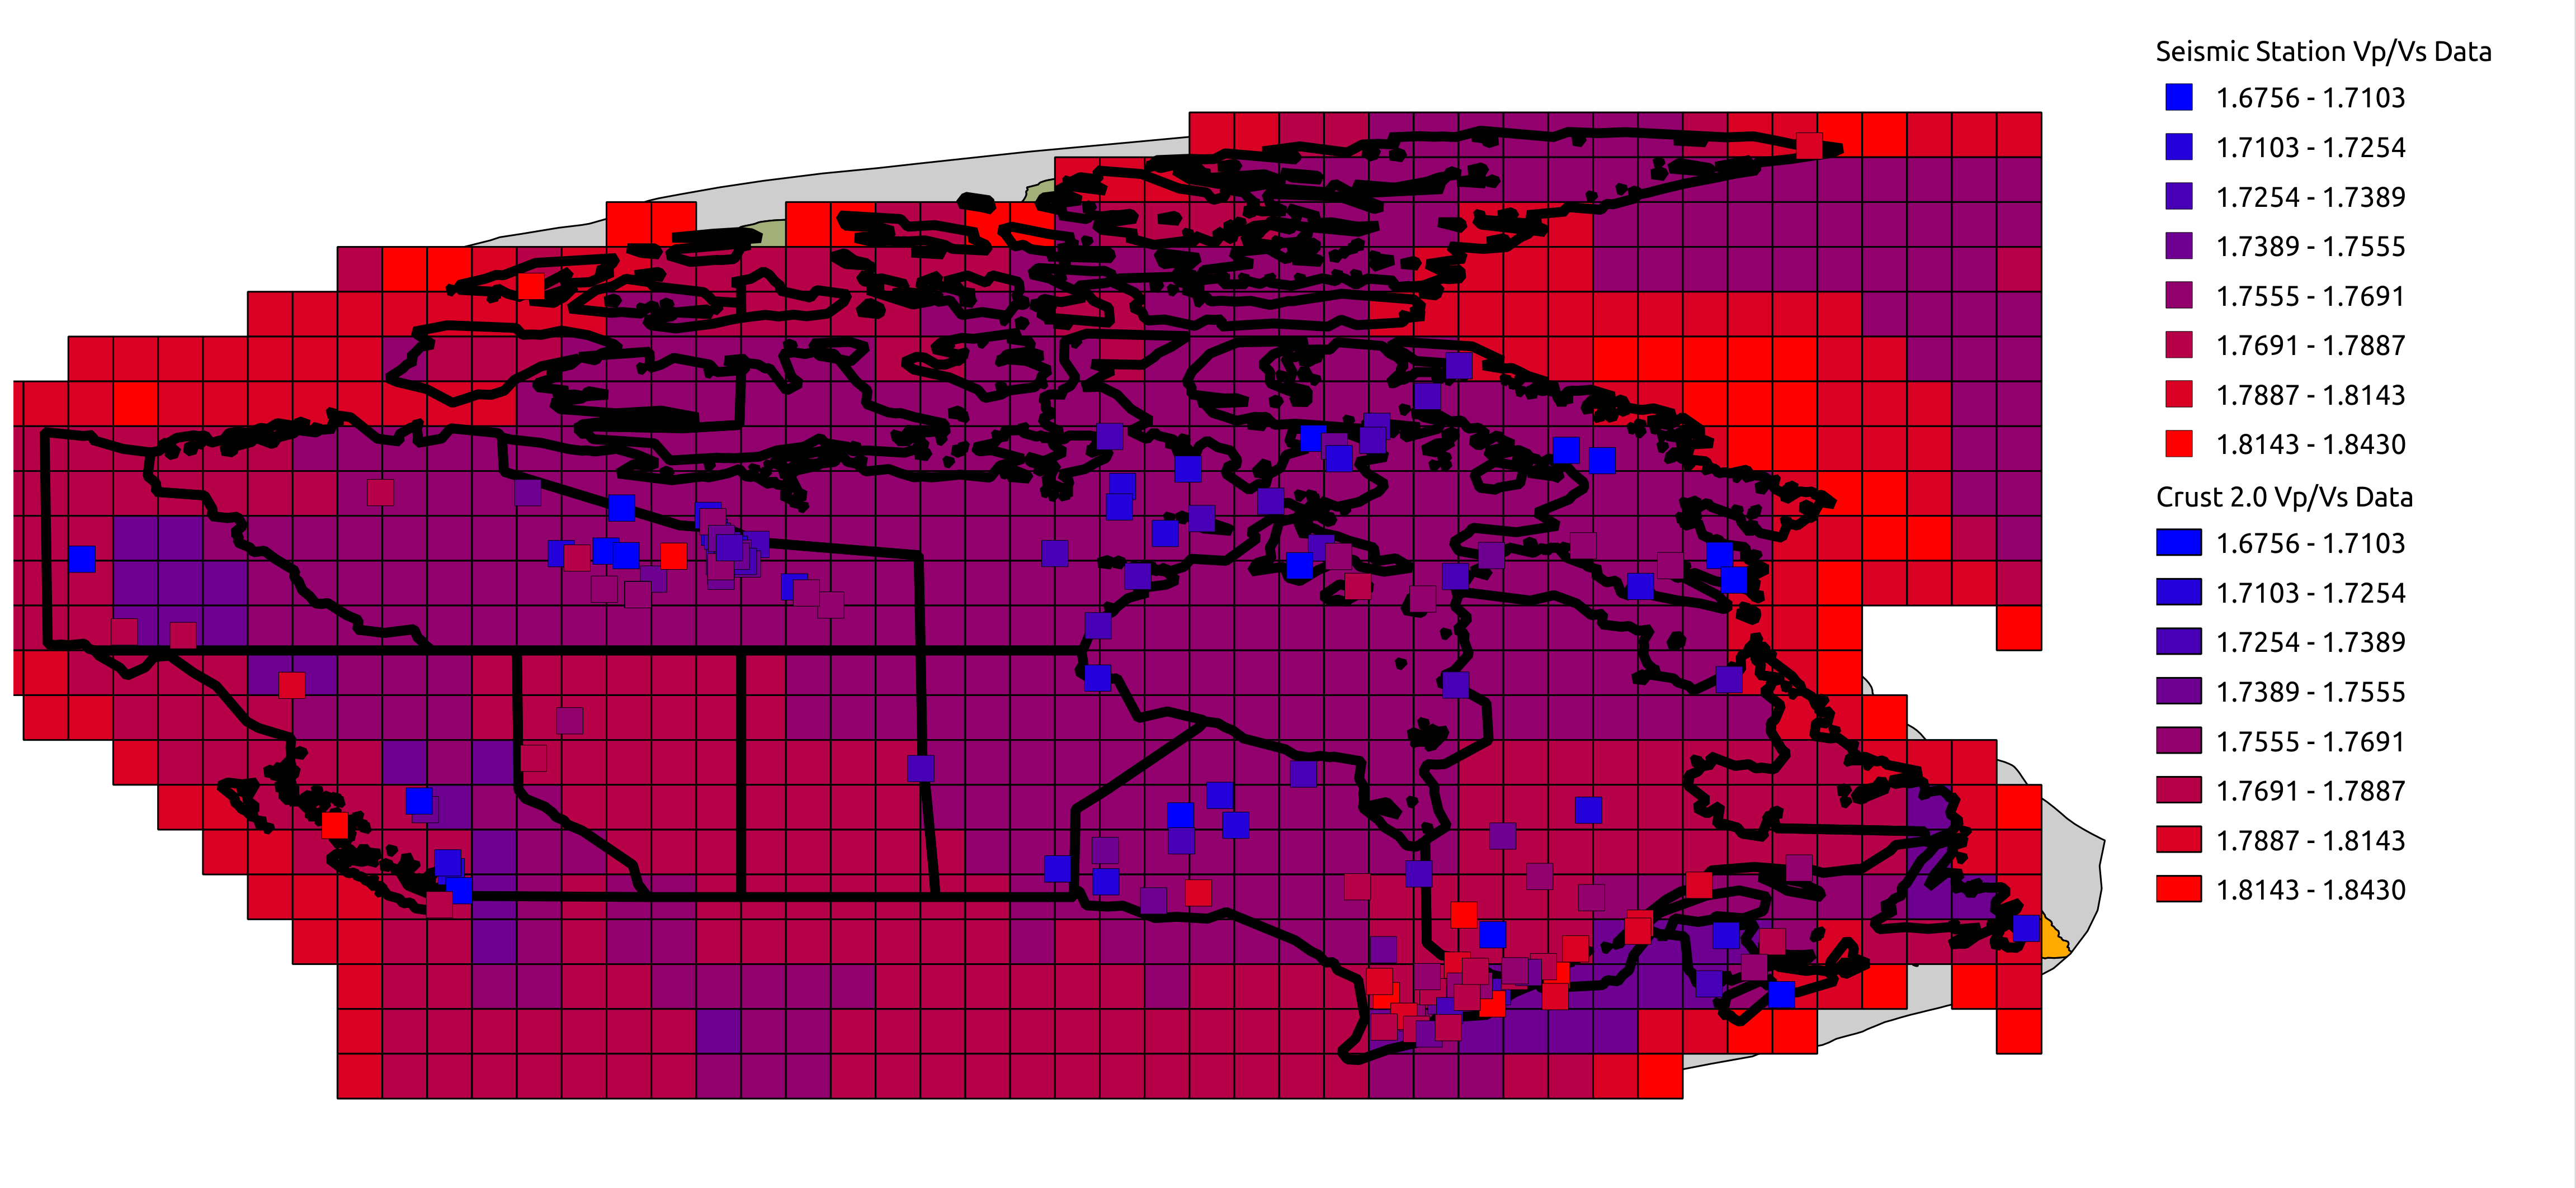
\includegraphics[width=\textwidth]{VpVsMapCrust}
  \caption{}
  \label{fig:VpVsMapCrust}
\end{figure}


%% -----------------------------------------------%%
\section{Discussion}
\subsection{Canada}

  The preliminary interrogation of the data set yields the observation that the bulk Canadian Shield has lower Vp/Vs than anticipated. Previous experiments show crustal averages of 1.77 (Christensen and Mooney, 1995) and 1.78 (Zandt and Ammon, 1995). This compares to computed values of 1.73, 1.74, 1.795 for the Churchill, Superior and Grenville Provinces Vp/Vs ratios respectively.


(MIGHT NOT INCLUDE)  The data bares out earlier results showing Proterozoic crust to have a higher seismic velocity ratio than Archean crust. This follows previous studies on crustal formation that have noted this trend in other regions (Durrheim and Mooney, 1991) . The increased crustal thickness of Proterozoic crust is clearly seen in the active source data while it not visible in data from processed seismic stations.

  Further work on the Bostock-Kumar stacking approach is warranted from a look at the cleanest stations. Before it can be employed in large scale analysis additional denoising methods or alternative deconvolution techniques will need to be investigated to reduce the noise in the data.


\subsection{Slave Province}
<Discussion on Slave Province>

%% -----------------------------------------------%%
\section{Conclusions}
<Conclusions here>

%% ------------------------------------------------------------------------ %%


\begin{thebibliography}
Bostock, M. G. (1998), Mantle stratigraphy and the evolution of the Slave province, J. Geophys. Res., 103, 21,183-21,200.

Bostock, M. G., M. R. Kumar (2010), Bias in seismic estimates of crustal properties, J. Geophys. Int., 182, 403-407.

Christensen, N. I. (1996), Poisson's ratio and crustal seismology, J. Geophys. Res., 101, 3139–3156.

Darbyshire, F. A., D. W. Eaton, A. W. Frederiksen, E. Leila (2006), New insights into the lithosphere beneath the Superior Province from Rayleigh wave dispersion and receiver function analysis, J. Geophys. Int., 169, 1043-1068.

Durrheim, R. J., W. D. Mooney (1991), Archean and Proterozoic crustal evolution, Geology, 19, 606-609.

Eaton, D. W., S. Dineva, R. Mereu (2005), Crustal thickness and Vp/Vs variations in the Grenville orogen (Ontario, Canada) from analysis of teleseismic receiver functions, Tectonophysics, 420, 223-238.

Efron, B., R. Tibshirani (1986), Bootstrap Methods for Standard Errors, Confidence Intervals, and Other Measures of Statistical Accuracy, Statistical Science, 1, 54-75.

Golub, G. H., M. Heath, G. Wahba (1979), Generalized cross-validation as a method for choosing a good ridge parameter, Technometrics, 21, 215-223.
Mooney, W. D. (2012), Personal communication. Compiled GSC active source data for the Canada.

Perry, H. K. C., D. W. S. Eaton, A. M. Forte (2002) LITH5.0: a revised crustal model for Canada based on Lithoprobe results,  J. Geophys. Int., 150, 285-294.

Thompson, D. A., I. D. Bastow, G. Helffrich, J.-M. Kendall, J. Wookey, D. B. Snyder, D. W. Eaton (2010), Precambrian crustal evolution: Seismic constraints from the Canadian Shield, Earth and Planetary Science Letters, 297, 655–666.

Zhu, L., H. Kanamori (2000), Moho depth variation in Southern California from teleseismic receiver functions, J. Geophys. Res., 105, 2969-2980.

Zandt, G., C. J. Ammon (1995), Continental crust composition constrained by measurements of crustal Poisson's ratio, Nature, 374, 152-154.

\end{thebibliography}


\end{document}

%% ------------------------------------------------------------------------ %%

